
%(BEGIN_QUESTION)
% Copyright 2010, Tony R. Kuphaldt, released under the Creative Commons Attribution License (v 1.0)
% This means you may do almost anything with this work of mine, so long as you give me proper credit

Sketch the wires necessary to connect two pressure switches and two relay coils to the following Allen-Bradley MicroLogix 1000 PLC (model 1761-L10BWA, with 6 discrete DC inputs either sourcing or sinking, and 4 discrete relay contact outputs).  Be sure to wire the two switches so they {\it source} current to the PLC's inputs (the low-pressure switch to {\tt I/2} and the high-pressure switch to {\tt I/5}, normally-open contacts on both) and wire the relay coils so the PLC {\it sources} current to them ({\tt O/0} and {\tt O/1}):

\vskip 50pt

$$\includegraphics[width=15.5cm]{i02379x01.eps}$$

\vfil

\underbar{file i02379}
\eject
%(END_QUESTION)





%(BEGIN_ANSWER)

This is a graded question -- no answers or hints given!

%(END_ANSWER)





%(BEGIN_NOTES)

Remember that ``sourcing'' means a device is sending current {\it out} through the channel wire (conventional flow notation), while ``sinking'' means a device is taking current {\it in} through the channel wire.  We ignore current through any ``Common'' conductors when we define source and sink, choosing only to reference conductors attached to specific input or output terminals of the device.

\vskip 10pt

In order for the process switches to source current to the PLC input channels, these switches must both connect to the positive pole of the DC power supply.  In other words, they must be ``high side'' switches, sending current (conventional flow notation) to the PLC input terminals.

\vskip 10pt

Likewise, in order for the PLC outputs to source current to the relay coils, the output contacts must both connect to the positive pole of the DC power supply.

$$\includegraphics[width=15.5cm]{i02379x02.eps}$$

% Note: the graphic image here (i02379x01.eps) is an ``exploded'' version of the 1761\_L10BWA Xcircuit object found in the plc.lps library file.  Use this as a starting point to create other MicroLogix 1000-series PLC objects!

%INDEX% PLC, I/O: discrete I/O device wiring

%(END_NOTES)


